\section{Thread Pool}
Thread Pool lösen das Problem, dass Threads sehr teuer sind. Ein Pool erledigt definierte Tasks, welche in einer definierten Anzahl Threads in dem Pool abgearbeitet werden.
Task sind potentielle Arbeitspakete (\textbf{run to completion}), welche reine passiv Objekte mit funktionaler Beschreibung.\\
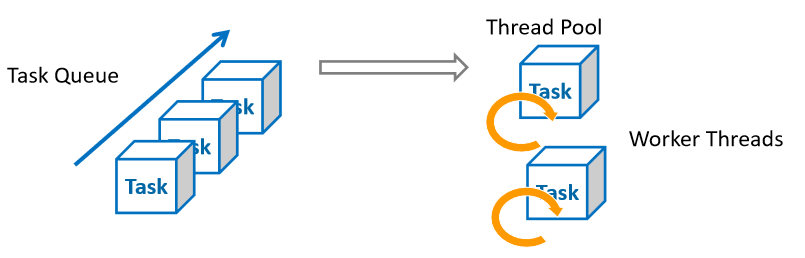
\includegraphics[width=\columnwidth]{Images/thread-pool}

\begin{lstlisting}
var pool = new ForkJoinPool();

// nicht blockierend
Future<Integer> future = pool.submit(() -> {
	// Task
	int value = ...;
	return value;
});
// oder
Integer future = pool.invoke(new MyRecursiveTask(value));

// blockierend
var res = future.get();
\end{lstlisting}
Beispiel um 3 Zahlen zu summieren welche nebeneinander in einem Array stehen.
\begin{lstlisting}
class ConvolutionTask extends RecursiveAction {
	private final int[] input;
	private final int[] output;
	private final int lower;
	private final int upper;
	private final static int THRESHOLD = 1000; // any value > 1
	public ConvolutionTask(int[] input, int[] output, int lower, int upper) {
		this.input = input;
		this.output = output;
		this.lower = lower;
		this.upper = upper;
	}
	@Override protected void compute() {
		if (upper - lower > THRESHOLD) {
			int middle = (lower + upper) / 2;
			invokeAll(
			new ConvolutionTask(input, output, lower, middle),
			new ConvolutionTask(input, output, middle, upper)
			);
		} else {
			for (int i = lower; i < upper; i++) {
				int left = i > 0 ? input[i - 1] : 0;
				int right = i < input.length - 1 ? input[i + 1] : 0;
				output[i] = left + input[i] + right;
			}
		}
	}
}
\end{lstlisting}

Ein \textbf{Daemon}-Thread hält das Programm nicht am leben. Daher müssen die Worker-Threads daemon sein, ansonsten würde das Programm nie beendet werden. Nachteil, Tasks sind nicht garantiert, dass sie abgearbeitet werden.


\subsection{Continuation}
\begin{lstlisting}
	CompletableFuture<Integer> future = CompletableFuture<Integer>.supplyAsync(()-> longOp());
	future.thenApply(result -> callWithReturn(result));
	future.thenAccept(result -> callNoReturn(result));
\end{lstlisting}


\subsection{.NET TPL}
In c\# gibt es eine Default Thread Pool welcher für 
\begin{enumerate}[nosep]
	\item Task: Explizite Tasks
	\item Data: Parallel Statements und Queries
	\item Asynchrone Programmierung
\end{enumerate}

\subsubsection{Parallel}
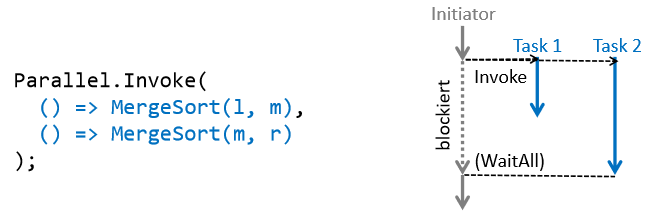
\includegraphics[width=\columnwidth]{Images/parallel_invoke}
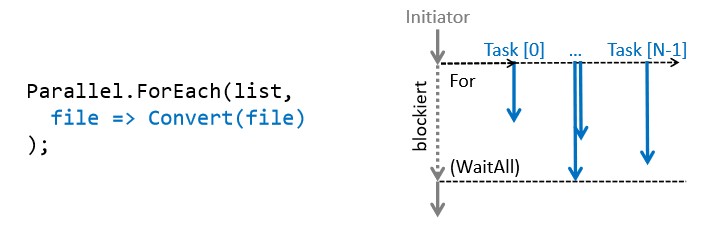
\includegraphics[width=\columnwidth]{Images/parallel_loop}
